\documentclass[10pt,a4paper]{article}
\usepackage[utf8]{inputenc}
\usepackage{amsmath}
\usepackage{amsfonts}
\usepackage{amssymb}
\usepackage{german}
\usepackage{graphicx}
\author{SEP - ITS - Team}
\title{Pflichtenheft}
\begin{document}
	\maketitle
	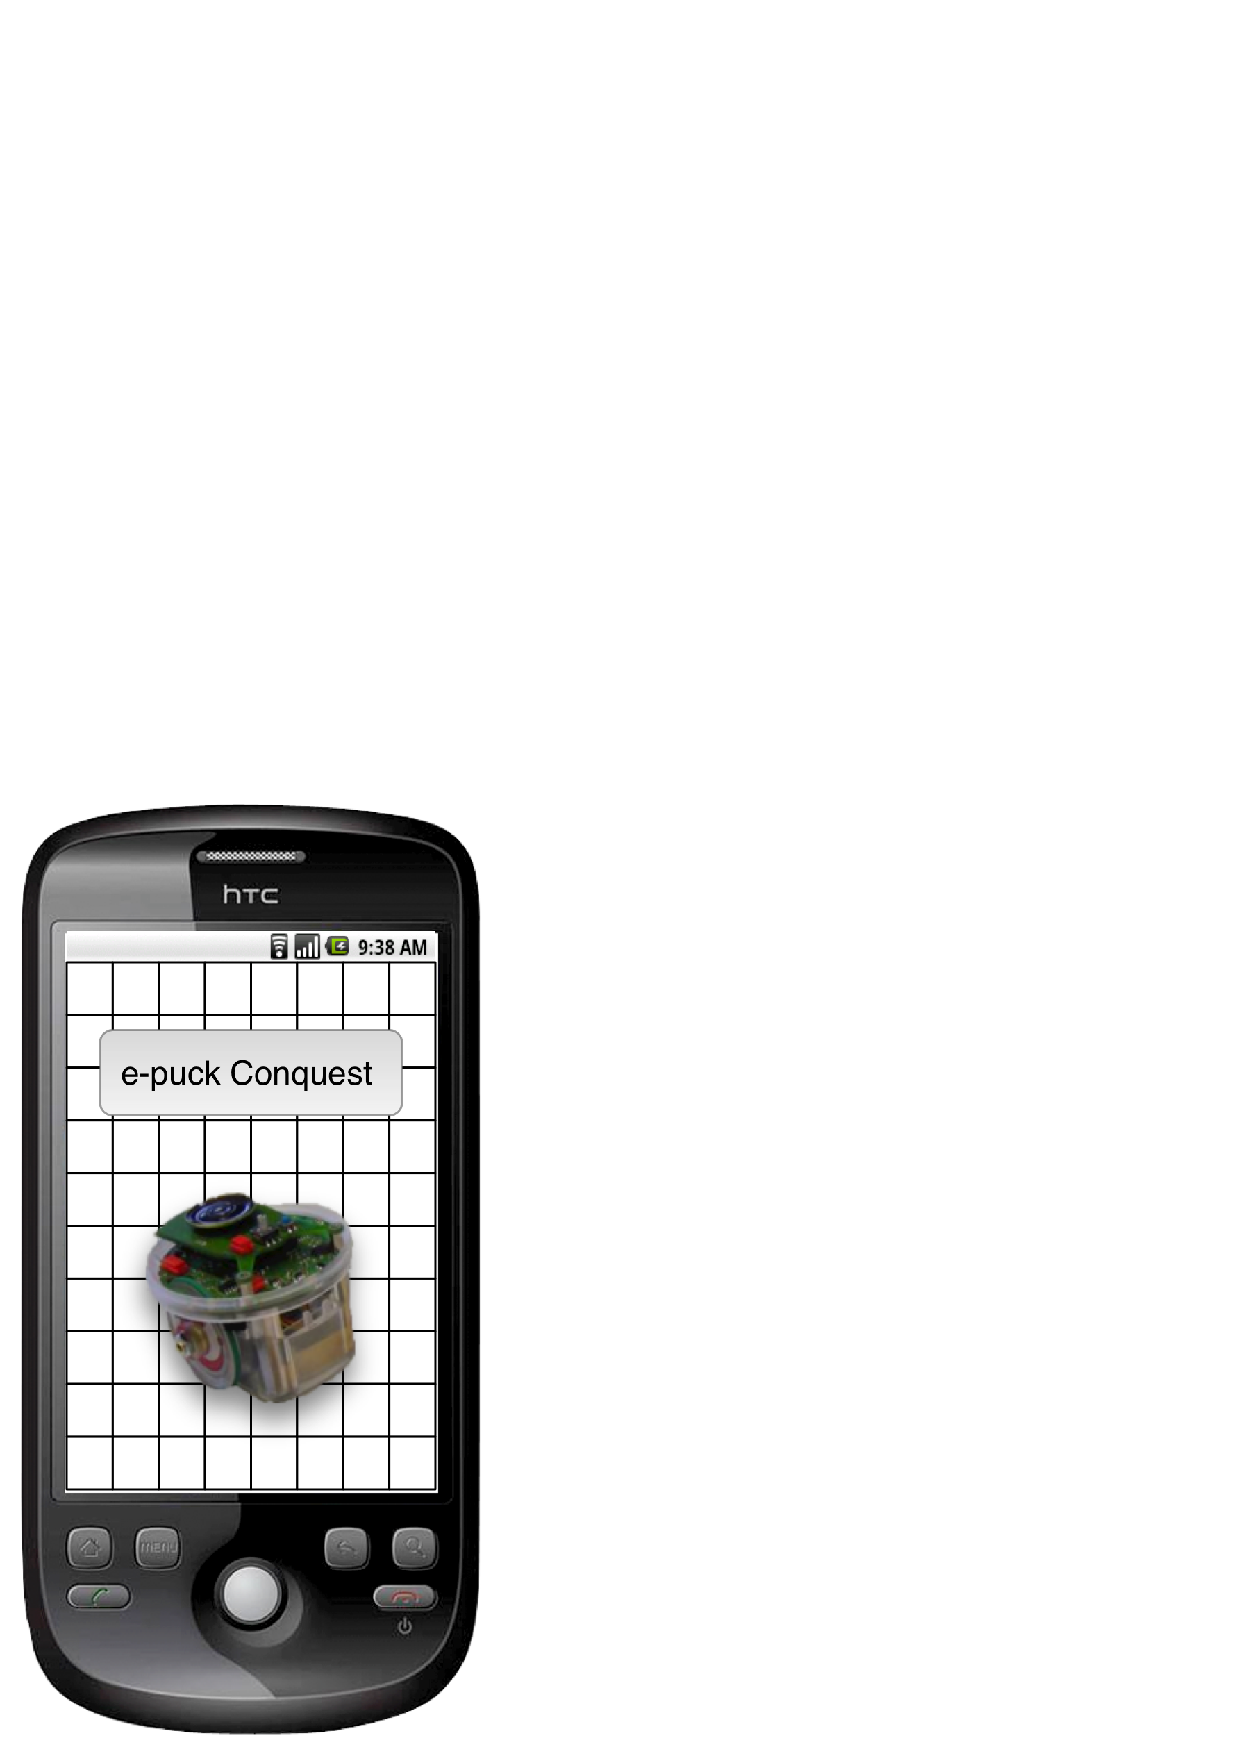
\includegraphics[scale=0.5, origin=c]{logo.png}
	\newpage
	\section{Zielbestimmung}
		Ziel des Projekts ist die autonome Erkundung eines unbekannten rechtwinkligen Spielfelds durch bis zu
		sechs e-puck Roboter. Dies wird durch Kooperation der Roboter und geeignete Algorithmen möglichst
		effizient umgesetzt. Zusätzlich erfolgt die kontinuierliche Visualisierung der Position der e-pucks auf der
		bereits erkundeten Karte mit einem Android-Smartphone. Die Steuerung eines Roboters kann wahlweise
		automatisch oder manuell per Smartphone erfolgen.
		\subsection{Musskriterien}
			\begin{itemize}
				\item e-puck Roboter
				\begin{itemize}
					\item Multiple Anzahl von Robotern
						\\ \textsl{Die Unterstützung von bis zu sechs e-puck Roboter muss gewährleistet sein.}
					\item Kommunikation über Bluetooth Netzwerk
					\item Erkundung einer unbekannten rechtwinkligen Fläche
						\\ \textsl{Das Spielfeld soll hierbei aus quadratischen Feldern bestehen. Diese sind rasterförmig
						 	und zusammenhängend angeordnet. Die Startpositionen der e-puck Roboter ist fest
						 	vordefiniert.}
					\item Fortbewegung auf den Kanten der Quadrate
						\\ \textsl{Die Linien müssen schwarz mit ausreichendem Kontrastverhältnis zum Untergrund
							sein.	Zwingend erforderlich ist, dass die Linienbreite innerhalb der Spezifikation der
							Bodensensoren	liegt.}		
					\item Kollisionsvermeidung
						\\ \textsl{Während der Erkundungsphase müssen die Roboter Kollisionen mit anderen Robotern
							bzw. Hindernissen vermeiden.}	
					\item Gleichberechtigung der Teilnehmer
						\\ \textsl{Sämtliche Roboter haben den selben Aufgabenbereich, auf eine Master/Slave-
							Beziehung wird verzichtet.}	
					\item Rückkehr zum Ausgangspunkt
						\\ \textsl{Nach vollendeter Erkundung müssen die e-pucks zurück zu ihrem jeweiligem
							Ausgangspunkt fahren.}	
				\end{itemize}
				\item Smartphone
				\begin{itemize}
					\item Kommunikation über Bluetooth
						\\ \textsl{Die Verbindung des Smartphones mit den Robotern muss über die vorhandenen
							Bluetooth Schnittstellen erfolgen.}
					\item Visualisierung
						\\ \textsl{Die bereits erkundete Karte muss inkl. der aktuellen Roboterpositionen in einer
							benutzerfreundlichen Android-Anwendung übersichtlich dargestellt werden.}		
					\item Steuerung des Roboters
						\\ \textsl{Es muss ein e-puck mit Hilfe der Anwendung gewählt werden können. Dieser lässt sich
							durch den Benutzer entlang der Kanten steuern. Die Richtung sowie Geschwindigkeit ist
							stufenweise anpassbar.}		
					\item Zwei Steuerungsarten
						\\ \textsl{Die Steuerung der Roboter erfolgt wahlweise über einen On-Screen- Joystick oder über
							den integrierten Beschleunigungssensor.}											
				\end{itemize}
			\end{itemize}
		\subsection{Wunschkriterien}
			\begin{itemize}
				\item e-puck Roboter
				\begin{itemize}
					\item Kritische Bereiche
					\item Beliebige Startpositionen
						\\ \textsl{Die Roboter können auf frei wählbaren Startpositionen innerhalb des Spielfeldes
							abgesetzt werden.}
					\item Zustandsvisualisierung	
					\item Einstellbarer Synchronisationsmodus
				\end{itemize}
				\item Smartphone
				\begin{itemize}
					\item Anzeige von Statusinformationen
					\item Pfadanzeige von einzelnen Robotern					
					\item Exportfunktion
					\item Internationalisierung										
				\end{itemize}
			\end{itemize}
		\subsection{Abgrenzungskriterien}
			\begin{itemize}
				\item Keine abweichenden Spielfelder
					\\ \textsl{Die Felder und zugehörigen Linien müssen den genannten Musskriterien
						entsprechen. Es sind keine runden oder diagonalen Verbindungslinien erlaubt.}
				\item Keine dynamischen Änderungen
					\\ \textsl{Nachdem der Erkundungsvorgang gestartet wurde, dürfen keine Modifikationen am
						Spielfeld getätigt werden, welche Einfluss auf den Erkundungsalgorithmus zur Folge haben.}			
				\item Maximal ein Smartphone
					\\ \textsl{Es darf lediglich ein Smartphone zur Auswahl, Steuerung und Visualisierung verwendet
						werden.}		
			\end{itemize}
	\section{Produkteinsatz}
		\subsection{Anwendungsbereiche}
			Das Projekt dient der Grundlagenforschung in den Bereichen:
			\begin{itemize}
				\item Robotik
				\item Verteilte Systeme
				\item Künstliche Intelligenz
			\end{itemize}
		\subsection{Zielgruppen}
			\begin{itemize}
				\item Studenten
				\item Forschungsgruppen in ähnlichen Bereichen
				\item e-puck Community
			\end{itemize}
		\subsection{Betriebsbedingungen}
			\begin{itemize}
				\item Ausreichende Stromversorgung
					\\ \textsl{ Die Akkuleistung der einzelnen Roboter sowie des Smartphones muss für die gesamte
						Erkundungsdauer ausreichend sein.}
				\item Geeignete Bedingungen für Funknetzwerke
					\\ \textsl{ Die Ausmaße des Spielfelds, die Abstände von e-pucks oder des Smartphones sowie
						Signale anderer Netze dürfen keine störenden Einflüsse auf die Bluetooth-Verbindungen haben.}
				\item Größe des Spielfeldes
					\\ \textsl{Der integrierte Arbeitsspeicher des e-puck Roboter stellt eine Begrenzung des 
					 persistierbaren lokalen Spielfeldes dar. Es werden ca. 700 Knotenpunkte unterstützt. }			
				\item Wartungsfrei
				\item Betriebsbedingungen des e-puck Roboter
					\\ \textsl{Die weiteren Betriebsbedingungen können dem Benutzerhandbuch 	entnommen werden.}
			\end{itemize}
<<<<<<< .mine
		\section{Produktumgebung}
			\subsection{Software}
				\begin{itemize}
					\item Geeigneter Bootloader oder Programmer zum Flashen der e-puck Roboter
					\item Android Software ab Version 2.1
				\end{itemize}
			\subsection{Hardware}
				\begin{itemize}
					\item e-puck Roboter
					\item Bodensensor für e-puck Roboter
					\item Android Smartphone
						\\ \textsl{Voraussetzungen: Bluetooth, geeignete Auflösung, Beschleunigungssensoren, Touch-Display.}
					\item Computer mit Bluetooth Unterstützung
				\end{itemize}		
	\section{Produktfunktionen}
		\subsection{e-puck Roboter}
			\subsubsection{Netzwerkfunktionen}
				\begin{list}{\labelitemi}{\leftmargin=1cm}
					\item[\textbf{\textbackslash F50\textbackslash}] Suchfunktion
					\item[\textbf{\textbackslash F60\textbackslash}] Verbindungsaufbau
					\item[\textbf{\textbackslash F70\textbackslash}] Broadcast-Kommunikation
					\item[\textbf{\textbackslash F75W\textbackslash}] Kommunikationsunterdrückung
				\end{list}
			\subsubsection{Bewegungsfunktionen}
				\begin{list}{\labelitemi}{\leftmargin=1cm}
					\item[\textbf{\textbackslash F80\textbackslash}] Fahrsteuerung 
					\item[\textbf{\textbackslash F90\textbackslash}] Kollisionsvermeidung
					\item[\textbf{\textbackslash F100\textbackslash}] Linienverfolgung
					\item[\textbf{\textbackslash F110\textbackslash}] Knotenanalyse
				\end{list}
			\subsubsection{Explorationsfunktionen}
				\begin{list}{\labelitemi}{\leftmargin=1cm}
					\item[\textbf{\textbackslash F120\textbackslash}] Lokalisierung 
					\item[\textbf{\textbackslash F130\textbackslash}] Lokale Kartenkonstruktion					
					\item[\textbf{\textbackslash F140\textbackslash}] Kartensynchronisation
					\item[\textbf{\textbackslash F150\textbackslash}] Erkundungsfunktion
					\item[\textbf{\textbackslash F160\textbackslash}] Rückkehrfunktion
					\item[\textbf{\textbackslash F170W\textbackslash}] Globale Lokalisierung (evtl. inkl. Steuerung)
				\end{list}
		\subsection{Smartphone}
			\subsubsection{Netzwerkfunktionen}
				\begin{list}{\labelitemi}{\leftmargin=1cm}
					\item[\textbf{\textbackslash F200\textbackslash}] Suchfunktion
					\item[\textbf{\textbackslash F210\textbackslash}] Verbindungsaufbau					
					\item[\textbf{\textbackslash F220\textbackslash}] Kommunikationsfunktion
				\end{list}				
			\subsubsection{GUI}
				\begin{list}{\labelitemi}{\leftmargin=1cm}
					\item[\textbf{\textbackslash F230\textbackslash}] Kartendarstellung
					\item[\textbf{\textbackslash F240\textbackslash}] Roboterdarstellung					
					\item[\textbf{\textbackslash F250\textbackslash}] Steuerungsfunktion per On-Screen-Joystick
					\item[\textbf{\textbackslash F260\textbackslash}] Steuerungsfunktion per Bewegungssensor					
					\item[\textbf{\textbackslash F270W\textbackslash}] Zustandsvisualisierung (status + pfade)		
					\item[\textbf{\textbackslash F280W\textbackslash}] Internationalisierung	
				\end{list}		
			\subsubsection{Steuerungsfunktionen}		
				\begin{list}{\labelitemi}{\leftmargin=1cm}
					\item[\textbf{\textbackslash F290\textbackslash}] Steuerungsfunktion per On-Screen-Joystick
					\item[\textbf{\textbackslash F300\textbackslash}] Steuerungsfunktion per Bewegungssensor					
				\end{list}				
=======
			
			
>>>>>>> .r8
\end{document}